%! Date = 2/22/24

\section{Introduction}\label{sec:introduction}
Larger Transformer~\cite{NEURIPS2017_3f5ee243} models achieve significantly better performance
~\cite{DBLP:journals/corr/abs-2005-14165, DBLP:journals/corr/abs-2001-08361},
hence the appeal for continuous scale.
However, this increase in model size demands exorbitant compute resources,
necessitating a distributed setting as memory requirements exceed the capacity of any
accelerator~\cite{DBLP:journals/corr/abs-2201-11990}
This interplay asks:
\emph{how do we sidestep the high costs of scaling Large Transformer models?}
\begin{figure}[!t]
    \begin{subfigure}{.5\linewidth}
        \centering
        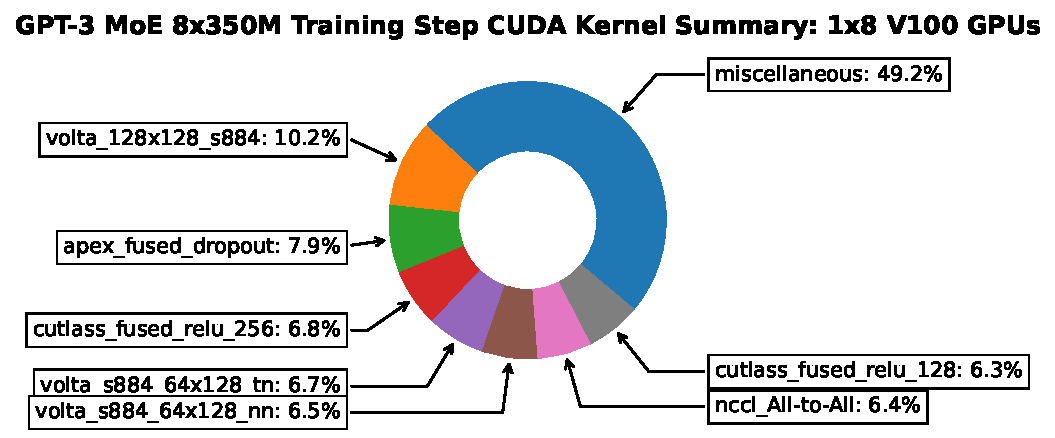
\includegraphics[width=0.9\linewidth]{images/single_trace_1x8_donut}
        \caption{NDv2 Node}
        \label{singlepie}
    \end{subfigure}\hfill % <-- "\hfill"
    \begin{subfigure}{.5\linewidth}
        \centering
        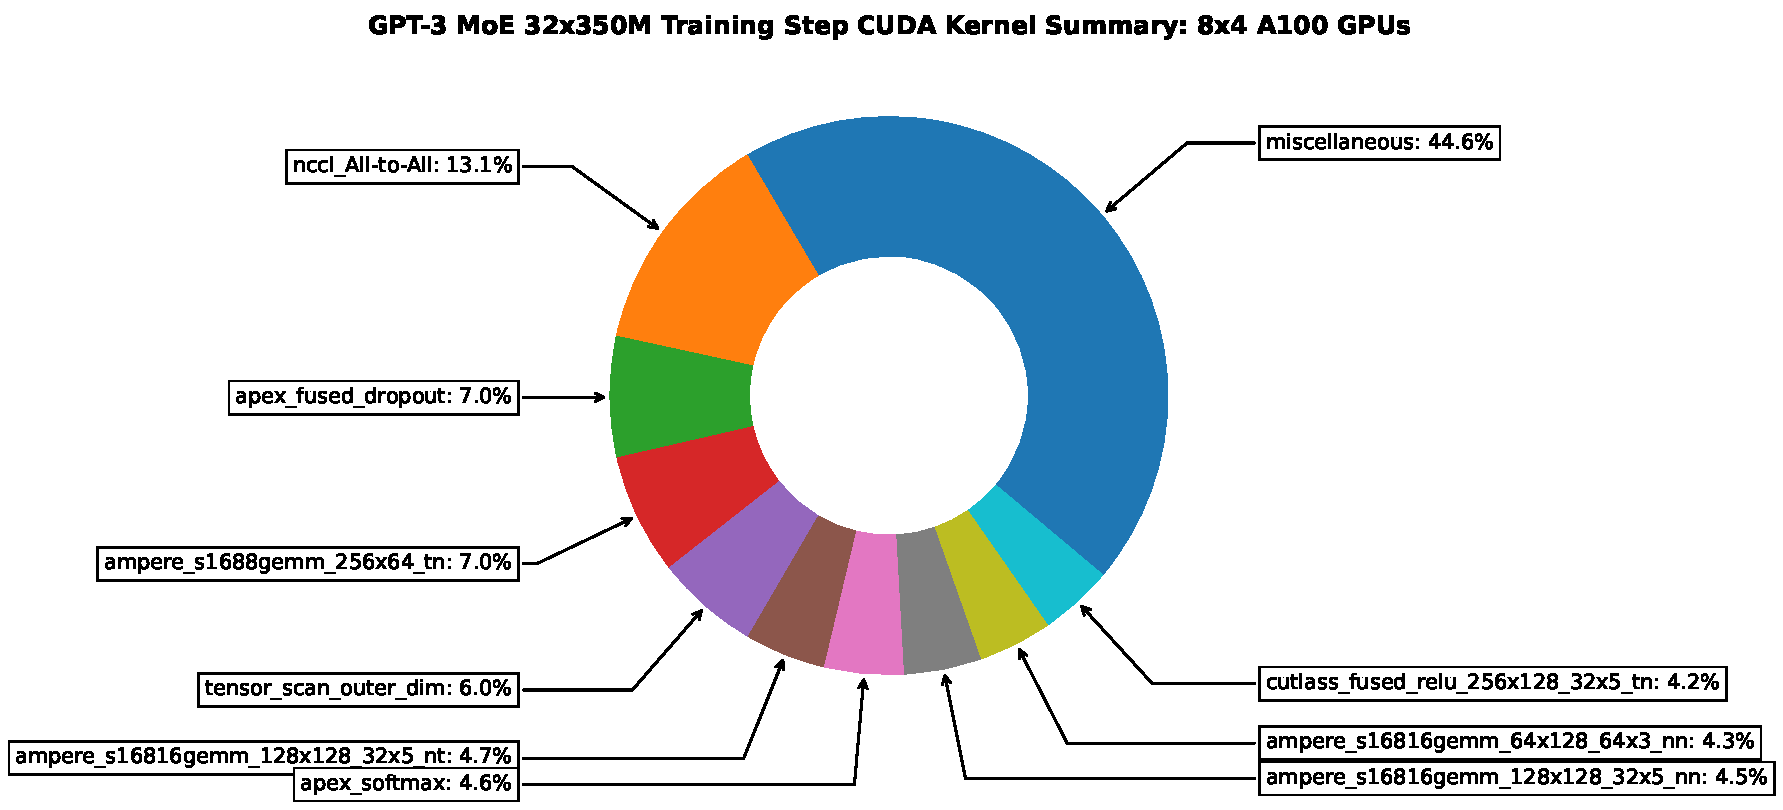
\includegraphics[width=\linewidth]{images/multi_sum_8x4_350M_donut}
        \caption{8 Perlmutter Nodes}
        \label{multi_350M_pie}
    \end{subfigure}
    \caption{\footnotesize DMoE Training Step CUDA Kernel Distribution.
    Observe in \ref{multi_350M_pie} that \emph{All-to-All} is the single most expensive operation.
    Note Perlmutter is a supercomputer.}
    \label{fig:donut}
\end{figure}
Current work shows the Mixture-of-Experts (MoE) architecture~\cite{ShazeerMMDLHD17},
based on ~\emph{conditional computation}~\cite{doi:10.1142/S0218001403002411}, is a productive answer.
For example, DeepSpeed of Microsoft shows 5x less training time for a GPT-3 MoE model at 1.3B and
7.3X faster inference for a trillion-parameter MoE model~\cite{pmlr-v162-rajbhandari22a}.
Notably, recently released Gemini 1.5, the first multimodal model to support context length of millions of tokens,
adopts this architecture~\cite{Gemini_Team_2024}.
On the other hand, this architecture introduces unsolved algorithmic and systems challenges,
such as load balancing across experts~\cite{ShazeerMMDLHD17}, training instability~\cite{NEURIPS2022_3e67e84a},
expert capacity restriction leading to token dropping~\cite{gale2022megablocks, DBLP:journals/corr/abs-2101-03961},
and collective communication overhead~\cite{DBLP:journals/corr/abs-2006-16668}.

In this work, we focus on the overhead of synchronous \emph{All-to-All},
specifically within NCCL~\cite{nccl} for GPU intercommunication and make the following contributions.
Firstly, we empirically demonstrate that the synchronous constraint of this
communication operation degrades performance by 1.6X up to 103X due to
the open \emph{straggler effect} problem~\cite{10.1145/2987550.2987554, deepspeedcomm}.
Next, we introduce Aristos, a distributed algorithm
that obviates this synchronous barrier, in favor of one-sided communication primitives and maximizes
concurrent overlap of communication and computation specifically for the MoE layer.
Also, we provide a sketch of a proof verifying the liveness property of Aristos.
In addition, we formulate an optimization for topology-aware expert parallelism
with the goal of minimizing communication and computation costs,
while satisfying memory and parallelism width constraints.
   
